\documentclass[12pt,a4paper]{article}

% Packages (typography & layout)
\usepackage[T1]{fontenc}
\usepackage{lmodern}
\usepackage{microtype}
\usepackage[dvipsnames]{xcolor}

\usepackage{amsmath,amssymb,amsthm}
\usepackage{geometry}
\usepackage{booktabs}
\usepackage{parskip}
\usepackage{fancyhdr}

\usepackage{tikz}
\usetikzlibrary{arrows.meta,positioning}

% Hyperlinks (load after most packages)
\usepackage{hyperref}

% Page setup
\geometry{margin=1in}
\setlength{\headheight}{15pt}

% Header/footer
\pagestyle{fancy}
\fancyhf{}
\fancyhead[L]{\textsc{Three Gates to Inevitability}}
\fancyhead[R]{\nouppercase{\leftmark}}
\fancyfoot[C]{\thepage}
\renewcommand{\headrulewidth}{0.4pt}
\renewcommand{\footrulewidth}{0pt}
\fancypagestyle{plain}{%
  \fancyhf{}
  \fancyfoot[C]{\thepage}
  \renewcommand{\headrulewidth}{0pt}
}

% Hyperref setup
\hypersetup{
    colorlinks=true,
    linkcolor=MidnightBlue,
    citecolor=MidnightBlue,
    urlcolor=MidnightBlue,
    pdfauthor={Jonathan Washburn},
    pdftitle={Three Gates to Inevitability},
    pdfsubject={Functional equations and cost composition},
    pdfkeywords={functional equation, d'Alembert, cosh, recognition composition law, RCL},
    bookmarksopen=true,
    bookmarksnumbered=true
}
\urlstyle{same}

% Small typography tweaks
\microtypesetup{protrusion=true, expansion=true}
\setlength{\emergencystretch}{2em}

% TikZ defaults
\tikzset{
  >={Stealth[length=2.2mm,width=1.4mm]},
  gate/.style={rectangle, rounded corners, draw=black!60, fill=black!3, minimum width=2.9cm, minimum height=1.05cm, align=center},
  result/.style={rectangle, rounded corners, draw=MidnightBlue!70, fill=MidnightBlue!8, thick, minimum width=4.3cm, minimum height=1.05cm, align=center}
}

% Theorem environments
\theoremstyle{plain}
\newtheorem{theorem}{Theorem}[section]
\newtheorem{lemma}[theorem]{Lemma}
\newtheorem{proposition}[theorem]{Proposition}
\newtheorem{corollary}[theorem]{Corollary}

\theoremstyle{definition}
\newtheorem{definition}[theorem]{Definition}
\newtheorem{hypothesis}[theorem]{Hypothesis}

\theoremstyle{remark}
\newtheorem{remark}[theorem]{Remark}

% Commands
\newcommand{\R}{\mathbb{R}}
\newcommand{\Rplus}{\mathbb{R}_{>0}}
\newcommand{\Jcost}{J}
\newcommand{\RCL}{\textup{RCL}}

\title{\vspace{-1cm}\textbf{Three Gates to Inevitability}\\[0.5em]
\large Characterizing the Recognition Composition Law via Functional Equations}
\author{Jonathan Washburn\\[0.3em]
Recognition Science Research Institute\\[0.5em]
\small Machine-verified in Lean 4 (\texttt{IndisputableMonolith})}
\date{January 2026}

\begin{document}

\maketitle


\begin{abstract}
We study multiplicatively consistent comparison costs $F:\Rplus\to\R$, i.e.\ those for which there exists an \emph{a priori} arbitrary combiner $P:\R^2\to\R$ satisfying
\[
F(xy)+F(x/y)=P(F(x),F(y))\qquad(x,y>0).
\]
A machine-verified counterexample shows that existence of \emph{some} such $P$ does not force the Recognition Composition Law (RCL), a calibrated form of the classical d'Alembert functional equation: the function $F(x)=\tfrac12(\log x)^2$ satisfies standard structural axioms yet admits the additive combiner $P(u,v)=2u+2v$.

We introduce three independently motivated ``gates''---interaction, entanglement, and curvature---that separate the canonical cost $J(x)=\tfrac12(x+x^{-1})-1$ from this counterexample family. We prove unconditionally that interaction forces entanglement, and that once $F=J$ the combiner is forced to be $P(u,v)=2uv+2u+2v$ on $[0,\infty)^2$ with \emph{no} regularity assumptions on $P$.

Finally, we isolate a single remaining analytic link---Hypothesis~\ref{hyp:bridge} (interaction $\Rightarrow$ hyperbolic ODE)---under which full inevitability follows: $F=J$ and $P$ is the RCL combiner. Core results are machine-verified in Lean 4.
\end{abstract}

\medskip
\noindent\textbf{2020 Mathematics Subject Classification.} 39B52 (Functional equations for functions with more general domains and/or ranges), 39B22 (Functional equations involving cosh and sinh).

\noindent\textbf{Keywords.} Functional equation, d'Alembert equation, multiplicative consistency, cosh, comparison cost, Lean 4.

\tableofcontents

\newpage

%==============================================================================
\section{Introduction}
%==============================================================================

\subsection{The Central Question}

Consider a fundamental mathematical structure: a \emph{cost function} $F(x)$ that measures how far a positive real number $x$ deviates from the reference value $1$. Such functions arise naturally in information theory (relative entropy, divergence measures) and the study of multiplicative groups \cite{Amari2000}. A natural question is: how should costs combine when we form products and quotients?

Specifically: if $x$ and $y$ each deviate from unity, how does the cost of the product $xy$ (and the quotient $x/y$) relate to the individual costs $F(x)$ and $F(y)$? We formalize this via \emph{multiplicative consistency}: the requirement that there exist a combiner function $P$ such that $F(xy)+F(x/y)=P(F(x),F(y))$.

The Recognition Composition Law (RCL) states that these costs combine as:
\begin{equation}\label{eq:RCL}
\Jcost(xy) + \Jcost(x/y) = 2\Jcost(x)\Jcost(y) + 2\Jcost(x) + 2\Jcost(y),
\end{equation}
where $\Jcost(x) = \frac{1}{2}(x + x^{-1}) - 1$. This is the multiplicative form of the classical \emph{d'Alembert functional equation} $f(t+u)+f(t-u)=2f(t)f(u)$, whose continuous solutions are $\cosh(\lambda t)$ for some $\lambda\in\R$ \cite{Aczel1966, Kuczma2009}. (This functional equation should not be confused with the d'Alembert wave equation $\partial^2 u/\partial t^2 = c^2\nabla^2 u$; the two are unrelated.)

Why \emph{this} law? The equation contains specific coefficients---all twos---and a specific coupling term $2\Jcost(x)\Jcost(y)$ that couples the two costs. What additional structure forces these coefficients?

Previous work established that the RCL is forced if one assumes the combiner is a low-degree polynomial. But critics correctly noted that this assumes too much about $P$. The polynomial restriction felt like smuggling in the answer.

\subsection{The Three Gates}

This paper takes a different approach. Instead of assuming properties of $P$, we identify three \emph{minimal physical requirements}---gates that a meaningful comparison law may be expected to satisfy. Each gate is independently motivated by physical intuition, and each is satisfied by the canonical cost while violated by the additive counterexample.

\begin{center}
{\small
\begin{tabular}{@{}clp{7cm}@{}}
\toprule
\textbf{Gate} & \textbf{Name} & \textbf{Physical meaning} \\
\midrule
1 & Interaction & The whole is not the sum of its parts \\
2 & Entanglement & Costs couple irreducibly, like quantum states \\
3 & Curvature & Log-coordinate geometry is hyperbolic \\
\bottomrule
\end{tabular}
}
\end{center}

The power of this approach is \emph{triangulation}: three independent lines of reasoning converge on the same target structure. Any alternative to the RCL must violate at least one of these gate conditions (or abandon multiplicative consistency altogether).

\subsection{The Counterexample}

A key motivation for this work is a counterexample showing that mere multiplicative consistency is insufficient to determine $P$.

The function
\[
F(x) = \frac{1}{2}(\log x)^2
\]
satisfies all structural axioms---symmetry under inversion, normalization at unity, smoothness, calibration---and admits a perfectly well-defined combiner $P(u,v) = 2u + 2v$. 

The combiner $P(u,v)=2u+2v$ is fundamentally different from the RCL combiner $P(u,v)=2uv+2u+2v$: it lacks the cross-term $2uv$.

This counterexample is machine-verified. It proves that the basic structural axioms alone are \emph{insufficient} to force the RCL. Additional conditions are needed---and the three gates formalize such conditions.

\begin{center}
{\small
\begin{tabular}{@{}lcc@{}}
\toprule
\textbf{Property} & \textbf{Canonical $\Jcost$} & \textbf{Counterexample} \\
\midrule
Interaction & \checkmark & $\times$ \\
Entanglement & \checkmark & $\times$ \\
Hyperbolic ODE & \checkmark & $\times$ \\
\bottomrule
\end{tabular}
}
\end{center}

The counterexample fails all three gates, while the canonical cost $\Jcost$ satisfies all three.

%==============================================================================
\section{Preliminaries}
%==============================================================================

\subsection{Definitions}

\begin{definition}[Cost Function]
\label{def:cost_function}
A \emph{cost function} $F: \Rplus \to \R$ measures the cost of deviation from unity, satisfying:
\begin{enumerate}
\item \textbf{Normalization}: $F(1) = 0$
\item \textbf{Symmetry}: $F(x) = F(1/x)$ for all $x > 0$
\item \textbf{Smoothness}: the log-lift $G(t)=F(e^t)$ is $C^2$ on $\R$
\item \textbf{Calibration}: $G''(0) = 1$ where $G(t) = F(e^t)$
\end{enumerate}
\end{definition}

\begin{definition}[Multiplicative Consistency]
$F$ is \emph{multiplicatively consistent} if there exists $P: \R^2 \to \R$ such that
\[
F(xy) + F(x/y) = P(F(x), F(y)) \quad \text{for all } x, y > 0.
\]
\end{definition}

\begin{definition}[Log-Lift]
For a cost function $F$, define $G: \R \to \R$ by $G(t) = F(e^t)$ and $H(t) = G(t) + 1$.
\end{definition}

\begin{lemma}[Symmetry implies an even log-lift]\label{lem:G_even}
If $F(x)=F(1/x)$ for all $x>0$ and $G(t)=F(e^t)$, then $G$ is even: $G(t)=G(-t)$ for all $t\in\R$.
In particular, if $G$ is differentiable at $0$ then $G'(0)=0$.
\end{lemma}

\begin{proof}
For any $t\in\R$,
\[
G(-t)=F(e^{-t})=F\!\left(\frac{1}{e^t}\right)=F(e^t)=G(t),
\]
so $G$ is even. If $G$ is differentiable at $0$, then
\[
G'(0)=\lim_{h\to 0}\frac{G(h)-G(0)}{h}
\quad\text{and}\quad
G'(0)=\lim_{h\to 0}\frac{G(-h)-G(0)}{-h},
\]
but $G(-h)=G(h)$ by evenness, so the two expressions differ by a minus sign; hence they must both equal $0$.
\end{proof}

\subsection{The Canonical Cost}

\begin{definition}[Canonical Cost]
$\Jcost(x) = \frac{1}{2}(x + x^{-1}) - 1$.
\end{definition}

The log-lift is $G_\Jcost(t) = \cosh(t) - 1$, and the RCL combiner is $P(u,v) = 2uv + 2u + 2v$.

%==============================================================================
\section{Gate 1: The Interaction Gate}
%==============================================================================

\subsection{Definition}

\begin{definition}[Interaction]
A cost function $F$ has \emph{interaction} if there exist $x, y > 0$ such that
\[
F(xy) + F(x/y) \neq 2F(x) + 2F(y).
\]
\end{definition}

The negation---no interaction---means $F(xy) + F(x/y) = 2F(x) + 2F(y)$ for all $x, y > 0$. In particular, if $F$ is multiplicatively consistent with some $P$, then on the range of $F$ the combiner behaves additively:
\[
P(F(x),F(y))=2F(x)+2F(y)\qquad(x,y>0).
\]

\subsection{Main Results}

\begin{theorem}[$\Jcost$ Has Interaction]\label{thm:J-interaction}
The canonical cost $\Jcost(x)=\frac12(x+x^{-1})-1$ has interaction. For example, at $x=y=2$:
\[
\Jcost(4) + \Jcost(1) \neq 2\Jcost(2) + 2\Jcost(2).
\]
\end{theorem}

\begin{proof}
We compute:
\[
\Jcost(1)=\tfrac12(1+1)-1=0,
\qquad
\Jcost(2)=\tfrac12\!\left(2+\tfrac12\right)-1=\tfrac54-1=\tfrac14,
\]
and
\[
\Jcost(4)=\tfrac12\!\left(4+\tfrac14\right)-1=\tfrac12\cdot\tfrac{17}{4}-1=\tfrac{17}{8}-1=\tfrac98.
\]
Therefore
\[
\Jcost(4)+\Jcost(1)=\tfrac98+0=\tfrac98
\quad\text{but}\quad
2\Jcost(2)+2\Jcost(2)=4\cdot\tfrac14=1,
\]
so $\Jcost(4)+\Jcost(1)\neq 2\Jcost(2)+2\Jcost(2)$. This witnesses interaction.
\end{proof}

\begin{theorem}[Counterexample Has No Interaction]\label{thm:Fquad-no-interaction}
Let $F(x) = \frac{1}{2}(\log x)^2$. Then for all $x, y > 0$:
\[
F(xy) + F(x/y) = 2F(x) + 2F(y).
\]
\end{theorem}

\begin{proof}
Direct calculation:
\begin{align*}
F(xy) + F(x/y) &= \frac{1}{2}(\log x + \log y)^2 + \frac{1}{2}(\log x - \log y)^2 \\
&= \frac{1}{2}[(\log x)^2 + 2\log x \log y + (\log y)^2] \\
&\quad + \frac{1}{2}[(\log x)^2 - 2\log x \log y + (\log y)^2] \\
&= (\log x)^2 + (\log y)^2 \\
&= 2F(x) + 2F(y). \qedhere
\end{align*}
\end{proof}

\subsection{Interpretation}

The interaction gate formalizes a notion of \emph{non-additivity}. In information geometry \cite{Amari2000}, additive cost functions correspond to flat manifolds (e.g., Euclidean metrics), while non-additive ones suggest curvature. The counterexample $F(x) = \frac{1}{2}(\log x)^2$ corresponds to the Euclidean squared distance in log-coordinates, representing a system where components decouple perfectly. The interaction gate rejects this flatness.

%==============================================================================
\section{Gate 2: The Entanglement Gate}
%==============================================================================

\subsection{Definition}

\begin{definition}[Entanglement]
\label{def:entanglement}
A combiner $P: \R^2 \to \R$ is \emph{entangling} if there exist $u_0, v_0, u_1, v_1 \in \R$ such that
\[
P(u_1, v_1) - P(u_1, v_0) - P(u_0, v_1) + P(u_0, v_0) \neq 0.
\]
This is the \emph{mixed second difference} \cite{AczelDhombres}, which for smooth $P$ approximates $\frac{\partial^2 P}{\partial u \partial v}$ (and equals it in the limit as the grid shrinks).
\end{definition}

\begin{definition}[Separability]
$P$ is \emph{separable} if $P(u, v) = \alpha(u) + \beta(v)$ for some functions $\alpha, \beta$.
\end{definition}

\begin{lemma}[Separability implies no entanglement]\label{lem:separable_not_entangling}
If $P$ is separable, then $P$ is not entangling; equivalently, if $P$ is entangling, then it is not separable.
\end{lemma}

\begin{proof}
Assume $P(u,v)=\alpha(u)+\beta(v)$. Then for any $u_0,u_1,v_0,v_1\in\R$ we have
\begin{align*}
&P(u_1,v_1)-P(u_1,v_0)-P(u_0,v_1)+P(u_0,v_0)\\
&\qquad=\bigl(\alpha(u_1)+\beta(v_1)\bigr)-\bigl(\alpha(u_1)+\beta(v_0)\bigr)-\bigl(\alpha(u_0)+\beta(v_1)\bigr)+\bigl(\alpha(u_0)+\beta(v_0)\bigr)=0.
\end{align*}
Hence no choice of $(u_0,v_0,u_1,v_1)$ yields a nonzero mixed second difference, so $P$ is not entangling.
\end{proof}

\begin{lemma}[A convenient form when $P$ is not entangling]\label{lem:not_entangling_decomp}
If $P$ is not entangling, then for all $u,v\in\R$,
\[
P(u,v)=P(u,0)+P(0,v)-P(0,0).
\]
In particular, $P$ is separable with $\alpha(u)=P(u,0)$ and $\beta(v)=P(0,v)-P(0,0)$.
\end{lemma}

\begin{proof}
``Not entangling'' means that for all $u_0,u_1,v_0,v_1\in\R$ the mixed second difference is zero:
\[
P(u_1,v_1)-P(u_1,v_0)-P(u_0,v_1)+P(u_0,v_0)=0.
\]
Apply this with $u_0=0$, $v_0=0$, $u_1=u$, $v_1=v$ to obtain
\[
P(u,v)-P(u,0)-P(0,v)+P(0,0)=0,
\]
which rearranges to the desired identity.
\end{proof}

\subsection{Main Results}

\begin{theorem}[RCL Is Entangling]\label{thm:RCL-entangling}
The RCL combiner $P(u,v) = 2uv + 2u + 2v$ is entangling:
\[
P(1,1) - P(1,0) - P(0,1) + P(0,0) = 6 - 2 - 2 + 0 = 2 \neq 0.
\]
\end{theorem}

\begin{proof}
Let $P(u,v)=2uv+2u+2v$. Taking $(u_0,v_0,u_1,v_1)=(0,0,1,1)$ gives
\[
P(1,1)-P(1,0)-P(0,1)+P(0,0)=6-2-2+0=2\neq 0,
\]
so $P$ is entangling by Definition~\ref{def:entanglement}.
\end{proof}

\begin{theorem}[Additive Combiner Is Not Entangling]\label{thm:Padd-not-entangling}
The combiner $P(u,v) = 2u + 2v$ is separable (hence not entangling):
\[
P(u_1, v_1) - P(u_1, v_0) - P(u_0, v_1) + P(u_0, v_0) = 0 \text{ for all } u_0, v_0, u_1, v_1.
\]
\end{theorem}

\begin{proof}
Write $P(u,v)=2u+2v=\alpha(u)+\beta(v)$ with $\alpha(u)=2u$ and $\beta(v)=2v$. By Lemma~\ref{lem:separable_not_entangling}, $P$ is not entangling.
\end{proof}

\begin{lemma}[Boundary values forced by the axioms]\label{lem:P_boundary_values}
Assume $F(1)=0$ and multiplicative consistency:
\[
F(xy)+F(x/y)=P(F(x),F(y))\qquad(x,y>0).
\]
Then for all $x>0$,
\[
P(F(x),0)=2F(x).
\]
If in addition $F$ is symmetric ($F(y)=F(1/y)$), then for all $y>0$,
\[
P(0,F(y))=2F(y).
\]
In particular, $P(0,0)=0$.
\end{lemma}

\begin{proof}
Set $y=1$ in multiplicative consistency. Since $F(1)=0$ and $x/1=x$, this gives
\[
F(x)+F(x)=P(F(x),F(1))=P(F(x),0),
\]
so $P(F(x),0)=2F(x)$.

Now set $x=1$. Then $1\cdot y=y$ and $1/y=y^{-1}$, so
\[
F(y)+F(y^{-1})=P(F(1),F(y))=P(0,F(y)).
\]
If $F$ is symmetric, $F(y^{-1})=F(y)$, hence $P(0,F(y))=2F(y)$. Finally, taking $x=y=1$ yields
\[
0=F(1)+F(1)=P(0,0).
\]
\end{proof}

\begin{theorem}[Interaction Forces Entanglement]\label{thm:interaction-entanglement}
Let $F$ be a cost function with symmetry, normalization, and multiplicative consistency with combiner $P$. If $F$ has interaction, then $P$ is entangling.
\end{theorem}

\begin{proof}
Assume, for contradiction, that $P$ is not entangling. By Lemma~\ref{lem:not_entangling_decomp}, for all $u,v\in\R$,
\[
P(u,v)=P(u,0)+P(0,v)-P(0,0).
\]
Apply this with $u=F(x)$ and $v=F(y)$. Using Lemma~\ref{lem:P_boundary_values} (which follows from normalization, symmetry, and consistency), we obtain for all $x,y>0$:
\[
P(F(x),F(y))=P(F(x),0)+P(0,F(y))-P(0,0)=2F(x)+2F(y)-0.
\]
By multiplicative consistency,
\[
F(xy)+F(x/y)=P(F(x),F(y))=2F(x)+2F(y)\qquad(x,y>0),
\]
which says $F$ has no interaction. This contradicts the interaction hypothesis. Therefore $P$ must be entangling.
\end{proof}

\subsection{Interpretation}

The entanglement gate formalizes non-separability at the level of the combiner. A combiner $P(u,v)$ is separable if it can be written as $\alpha(u)+\beta(v)$ for some functions $\alpha,\beta$; otherwise it is entangling. This condition is related to the vanishing of the mixed partial derivative $\partial^2 P/\partial u \partial v$.

The RCL combiner is:
\[
P(u,v) = 2uv + 2u + 2v.
\]
The cross-term $2uv$ ensures $\partial^2 P/\partial u \partial v = 2 \neq 0$. This coupling is essential for any theory where the cost of a composite system depends on the interaction between its components.

The counterexample's combiner $P(u,v) = 2u + 2v$ is separable ($\partial^2 P = 0$). It factors into independent contributions. By Theorem~\ref{thm:interaction-entanglement}, this separability is precisely why the counterexample lacks interaction.

%==============================================================================
\section{Gate 3: The Curvature Gate}
%==============================================================================

\subsection{ODE Classification}

Gate~3 is a geometric closure condition. Rather than deriving an ODE from multiplicative consistency (the remaining analytic gap), we postulate that the recognition metric in log-coordinates has constant curvature; in our formalization this is captured by one of three canonical ODE types for the log-lift $G(t)=F(e^t)$:

\begin{definition}[Curvature Types]
\label{def:curvature_types}
\begin{enumerate}
\item \textbf{Flat} ($\kappa = 0$): $G''(t) = 1$ for all $t$
\item \textbf{Hyperbolic} ($\kappa = -1$): $G''(t) = G(t) + 1$ for all $t$
\item \textbf{Spherical} ($\kappa = +1$): $G''(t) = -(G(t) + 1)$ for all $t$
\end{enumerate}
\end{definition}

\subsection{Main Results}

\begin{theorem}[Canonical Cost Is Hyperbolic]\label{thm:J-hyperbolic}
Let $G(t) = \cosh(t) - 1$. Then $G''(t) = \cosh(t) = G(t) + 1$.
\end{theorem}

\begin{proof}
We have $G'(t)=\sinh(t)$ and $G''(t)=\cosh(t)$. Since $G(t)+1=\cosh(t)-1+1=\cosh(t)$, it follows that $G''(t)=G(t)+1$ for all $t$.
\end{proof}

\begin{theorem}[Counterexample Is Flat]\label{thm:Fquad-flat}
Let $G(t) = t^2/2$. Then $G''(t) = 1$.
\end{theorem}

\begin{proof}
Differentiate: $G'(t)=t$ and $G''(t)=1$ for all $t$.
\end{proof}

\begin{lemma}[Flat ODE forces the quadratic log-cost]\label{lem:flat_forces_quad}
Let $G:\R\to\R$ be twice differentiable and assume
\[
G''(t)=1\ \text{for all }t\in\R,\qquad G(0)=0,\qquad G'(0)=0.
\]
Then $G(t)=t^2/2$ for all $t\in\R$. Consequently, the associated cost function $F(x)=G(\log x)$ satisfies $F(x)=\tfrac12(\log x)^2$.
\end{lemma}

\begin{proof}
Integrating $G''(t)=1$ gives $G'(t)=t+C$ for some constant $C$. Evaluating at $t=0$ yields $0=G'(0)=C$, hence $G'(t)=t$.
Integrating again gives $G(t)=t^2/2+D$ for some constant $D$. Evaluating at $t=0$ yields $0=G(0)=D$, hence $G(t)=t^2/2$.
The final statement follows by substitution $t=\log x$.
\end{proof}

\begin{theorem}[Spherical Is Ruled Out by Calibration]\label{thm:spherical-ruled-out}
If $G''(t) = -(G(t) + 1)$ and $G(0) = 0$, then $G''(0) = -1$. But calibration requires $G''(0) = 1$. Contradiction.
\end{theorem}

\begin{proof}
Evaluate the ODE at $t=0$:
\[
G''(0)=-(G(0)+1)=-(0+1)=-1.
\]
This contradicts the calibration requirement $G''(0)=1$.
\end{proof}

\begin{corollary}[Curvature Dichotomy]
Among the three constant-curvature ODE types in Definition~\ref{def:curvature_types}, calibration rules out the spherical case. Thus the remaining possibilities are:
\begin{enumerate}
\item Flat ($G'' = 1$): the counterexample family
\item Hyperbolic ($G'' = G + 1$): the canonical cost
\end{enumerate}
\end{corollary}

\begin{proof}
By Theorem~\ref{thm:spherical-ruled-out}, the spherical ODE $G''=-(G+1)$ is incompatible with calibration $G''(0)=1$ (and $G(0)=0$). Therefore only the flat and hyperbolic ODE types remain among the three listed in Definition~\ref{def:curvature_types}.
\end{proof}

\subsection{Interpretation}

The curvature gate is naturally interpreted in the context of \emph{information geometry}, where cost functions induce metric structures on probability manifolds.

The three ODE families correspond to the three constant-curvature geometries in 1D:
\begin{itemize}
\item \textbf{Flat} ($\kappa = 0$): $G(t) \sim t^2$. Euclidean geometry. This corresponds to the Gaussian (normal) distribution with fixed variance, where the Fisher information metric is flat.
\item \textbf{Hyperbolic} ($\kappa = -1$): $G(t) \sim \cosh t$. Hyperbolic geometry. This structure appears in the study of exponential families and the geometry of statistical manifolds \cite{Amari2000}.
\item \textbf{Spherical} ($\kappa = +1$): $G(t) \sim \cos t$. Spherical geometry.
\end{itemize}

The counterexample corresponds to the flat case. Interaction rules out this flatness, forcing the geometry to be non-Euclidean. Calibration then selects the hyperbolic branch over the spherical one.

%==============================================================================
\section{The Triangulated Proof}
%==============================================================================

\subsection{Convergence}

The three gates were developed independently, motivated by different intuitions: holism (Gate 1), quantum non-separability (Gate 2), and geometric curvature (Gate 3). Yet they converge on the same dichotomy.

\begin{theorem}[Gates Are Consistent]\label{thm:gates-consistent}
The canonical cost $\Jcost$ passes all three gates:
\begin{enumerate}
\item $\Jcost$ has interaction (the whole exceeds the sum)
\item The RCL combiner is entangling (costs couple irreducibly)
\item The log-lift $\cosh(t) - 1$ satisfies the hyperbolic ODE (curved geometry)
\end{enumerate}
The counterexample fails all three gates:
\begin{enumerate}
\item $F_{\text{quad}}$ has no interaction (perfectly decomposable)
\item The additive combiner is not entangling (separable)
\item The log-lift $t^2/2$ satisfies the flat ODE (Euclidean geometry)
\end{enumerate}
\end{theorem}

\begin{proof}
For the canonical cost $\Jcost$, Theorem~\ref{thm:J-interaction} proves interaction. Theorem~\ref{thm:RCL-entangling} proves that the RCL combiner is entangling. Theorem~\ref{thm:J-hyperbolic} proves that its log-lift $G(t)=\cosh(t)-1$ satisfies the hyperbolic ODE.

For the counterexample $F(x)=\tfrac12(\log x)^2$, Theorem~\ref{thm:Fquad-no-interaction} proves no interaction. Theorem~\ref{thm:Padd-not-entangling} proves the additive combiner $P(u,v)=2u+2v$ is not entangling. Theorem~\ref{thm:Fquad-flat} proves the log-lift $G(t)=t^2/2$ satisfies the flat ODE.
\end{proof}

This consistency is not a coincidence. The three gates are \emph{perspectives on the same structure}---interaction, entanglement, and curvature are three faces of the same geometric solid.

\subsection{The Bridge Hypothesis}

The three gates are logically connected, and we have machine-verified all but one link in the chain. The remaining link is:

\begin{hypothesis}[Interaction Forces Hyperbolic ODE]\label{hyp:bridge}
If $F$ satisfies the structural axioms (symmetry, normalization, smoothness, calibration) and has interaction, then its log-lift $G$ satisfies $G''(t) = G(t) + 1$.
\end{hypothesis}

This hypothesis asserts that interaction alone---the requirement that the whole exceed the sum of its parts---is sufficient to force hyperbolic geometry. It is the keystone of the triangulated proof.

Under this hypothesis, the logical chain is:
\begin{enumerate}
\item \textbf{Interaction $\Rightarrow$ Hyperbolic ODE} (the bridge hypothesis)
\item \textbf{Hyperbolic ODE + calibration $\Rightarrow$ $G = \cosh - 1$} (ODE uniqueness---machine-verified)
\item \textbf{$G = \cosh - 1$ $\Rightarrow$ $F = \Jcost$} (by definition of log-lift)
\item \textbf{$F = \Jcost$ $\Rightarrow$ $P = $ RCL} (unconditional---machine-verified with \emph{no} assumptions on $P$)
\end{enumerate}

The bridge hypothesis is the only remaining conjecture. Every other step is either definitional or machine-verified.

\subsection{Two Standard Links (Expanded Proofs)}

For completeness, we now expand two links in the chain that are often treated as ``standard'' and left implicit: (i) solving the hyperbolic ODE, and (ii) forcing the combiner once $F=\Jcost$. (Both are also machine-verified in our Lean development.)

\begin{proposition}[Hyperbolic ODE forces the canonical log-lift]\label{prop:hyperbolic_forces_cosh}
Let $G:\R\to\R$ be twice differentiable and assume
\[
G''(t)=G(t)+1 \quad\text{for all } t\in\R,
\qquad
G(0)=0,
\qquad
G'(0)=0.
\]
Then $G(t)=\cosh(t)-1$ for all $t\in\R$.
\end{proposition}

\begin{proof}
Define $H(t)=G(t)+1$. Then $H''(t)=H(t)$ for all $t$, and the initial conditions become $H(0)=1$ and $H'(0)=0$.

Since $H''=H$ is a constant-coefficient linear ODE, its general $C^2$ solution has the form (see, e.g., \cite{BoyceDiPrima})
\[
H(t)=Ae^{t}+Be^{-t}
\]
for constants $A,B\in\R$. Differentiating gives $H'(t)=Ae^{t}-Be^{-t}$, so the initial conditions yield
\[
H(0)=A+B=1,\qquad H'(0)=A-B=0.
\]
Thus $A=B=\tfrac12$ and therefore
\[
H(t)=\tfrac12(e^{t}+e^{-t})=\cosh(t).
\]
Finally, $G(t)=H(t)-1=\cosh(t)-1$.
\end{proof}

\begin{lemma}[$\Jcost$ satisfies the RCL identity]\label{lem:Jcost_satisfies_RCL}
For all $x,y>0$,
\[
\Jcost(xy)+\Jcost(x/y)=2\Jcost(x)\Jcost(y)+2\Jcost(x)+2\Jcost(y).
\]
\end{lemma}

\begin{proof}
Write $\Jcost(x)=\frac12(x+x^{-1})-1$. Let $a=x+x^{-1}$ and $b=y+y^{-1}$. Then
\[
\Jcost(x)=\tfrac12(a-2),\qquad \Jcost(y)=\tfrac12(b-2).
\]
First compute the left-hand side:
\begin{align*}
\Jcost(xy)+\Jcost(x/y)
&=\left(\tfrac12(xy+(xy)^{-1})-1\right)+\left(\tfrac12(x/y+y/x)-1\right)\\
&=\tfrac12\!\left(xy+\frac{x}{y}+\frac{y}{x}+\frac{1}{xy}\right)-2.
\end{align*}
Next compute the right-hand side:
\begin{align*}
2\Jcost(x)\Jcost(y)+2\Jcost(x)+2\Jcost(y)
&=2\cdot\tfrac12(a-2)\cdot\tfrac12(b-2)+(a-2)+(b-2)\\
&=\tfrac12(a-2)(b-2)+a+b-4\\
&=\tfrac12(ab-2a-2b+4)+a+b-4\\
&=\tfrac12ab-2.
\end{align*}
Finally, expand $ab=(x+x^{-1})(y+y^{-1})=xy+\frac{x}{y}+\frac{y}{x}+\frac{1}{xy}$, so the two expressions match.
\end{proof}

\begin{lemma}[Surjectivity of $\Jcost$ onto $[0,\infty)$]\label{lem:Jcost_surjective}
For every $u\ge 0$ there exists $x>0$ with $\Jcost(x)=u$. In fact, one may take
\[
x=(1+u)+\sqrt{u(u+2)}.
\]
\end{lemma}

\begin{proof}
For $x>0$ we rewrite
\[
\Jcost(x)=\tfrac12(x+x^{-1})-1=\tfrac12\left(\frac{x^2+1-2x}{x}\right)=\frac{(x-1)^2}{2x}.
\]
Fix $u\ge 0$ and solve $\Jcost(x)=u$:
\[
u=\frac{(x-1)^2}{2x}\quad\Longleftrightarrow\quad x^2-2(1+u)x+1=0.
\]
By the quadratic formula,
\[
x=(1+u)\pm\sqrt{(1+u)^2-1}=(1+u)\pm\sqrt{u(u+2)}.
\]
Both roots are positive; choosing the $+$ sign gives the stated $x>0$ with $\Jcost(x)=u$.
\end{proof}

\begin{theorem}[Unconditional forcing of the RCL combiner once $F=\Jcost$]\label{thm:P_forced_from_J}
Let $P:\R^2\to\R$ be any function satisfying multiplicative consistency with $\Jcost$:
\[
\Jcost(xy)+\Jcost(x/y)=P(\Jcost(x),\Jcost(y))\qquad(x,y>0).
\]
Then for all $u,v\ge 0$,
\[
P(u,v)=2uv+2u+2v.
\]
No regularity assumptions on $P$ are required.
\end{theorem}

\begin{proof}
Fix $u,v\ge 0$. By Lemma~\ref{lem:Jcost_surjective}, choose $x,y>0$ such that $\Jcost(x)=u$ and $\Jcost(y)=v$. Then by consistency,
\[
P(u,v)=P(\Jcost(x),\Jcost(y))=\Jcost(xy)+\Jcost(x/y).
\]
By Lemma~\ref{lem:Jcost_satisfies_RCL}, the right-hand side equals
\[
2\Jcost(x)\Jcost(y)+2\Jcost(x)+2\Jcost(y)=2uv+2u+2v.
\]
\end{proof}

\begin{theorem}[Full inevitability (conditional on the bridge)]\label{thm:full_inevitability}
Let $F:\Rplus\to\R$ be a cost function in the sense of Definition~\ref{def:cost_function}, and assume $F$ is multiplicatively consistent with some $P:\R^2\to\R$.
If $F$ has interaction and Hypothesis~\ref{hyp:bridge} holds, then:
\begin{enumerate}
\item $F(x)=\Jcost(x)$ for all $x>0$, and
\item for all $u,v\ge 0$, $P(u,v)=2uv+2u+2v$.
\end{enumerate}
\end{theorem}

\begin{proof}
Let $G(t)=F(e^t)$. Since $F(1)=0$, we have $G(0)=0$.
By symmetry and Lemma~\ref{lem:G_even}, $G$ is even and hence $G'(0)=0$.

Because $F$ has interaction, Hypothesis~\ref{hyp:bridge} implies that $G$ satisfies the hyperbolic ODE $G''(t)=G(t)+1$ for all $t$.
By Proposition~\ref{prop:hyperbolic_forces_cosh}, it follows that $G(t)=\cosh(t)-1$ for all $t$.

Therefore, for $x>0$,
\[
F(x)=G(\log x)=\cosh(\log x)-1=\frac{e^{\log x}+e^{-\log x}}{2}-1=\frac{x+x^{-1}}{2}-1=\Jcost(x).
\]
This proves (1).

For (2), since $F=\Jcost$ and $F$ is multiplicatively consistent with $P$, we have
\[
\Jcost(xy)+\Jcost(x/y)=P(\Jcost(x),\Jcost(y))\qquad(x,y>0).
\]
Applying Theorem~\ref{thm:P_forced_from_J} yields $P(u,v)=2uv+2u+2v$ for all $u,v\ge 0$.
\end{proof}

\begin{remark}
The conclusion $P(u,v)=2uv+2u+2v$ is asserted on $[0,\infty)^2$, i.e.\ on the range of $(\Jcost(x),\Jcost(y))$. No claim is made about values of $P$ outside this set, which are unconstrained by multiplicative consistency with $F=\Jcost$.
\end{remark}

\subsection{The Triangulated Structure}

\begin{center}
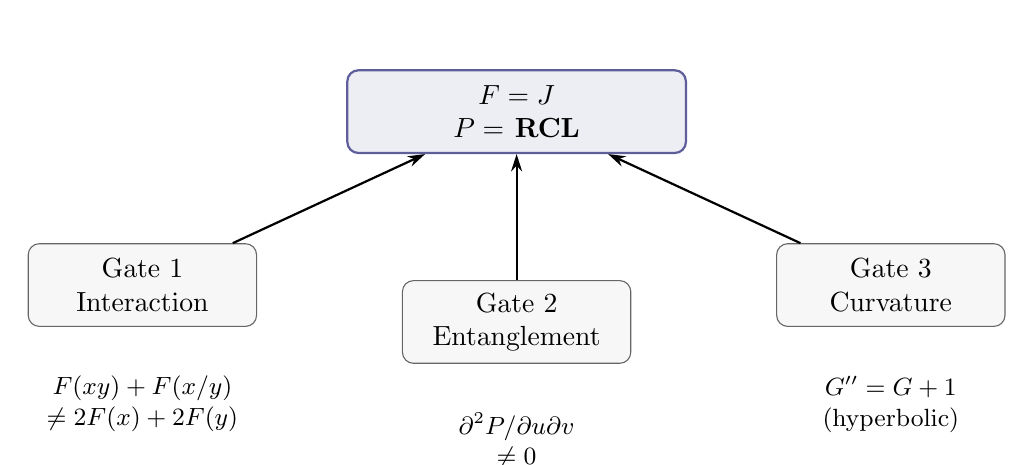
\begin{tikzpicture}[node distance=1.6cm]
\node[result] (conclusion) {\textbf{$F=\Jcost$}\\\textbf{$P=$ RCL}};
\node[gate, below left=of conclusion] (gate1) {Gate 1\\Interaction};
\node[gate, below=of conclusion] (gate2) {Gate 2\\Entanglement};
\node[gate, below right=of conclusion] (gate3) {Gate 3\\Curvature};

\draw[->, thick] (gate1) -- (conclusion);
\draw[->, thick] (gate2) -- (conclusion);
\draw[->, thick] (gate3) -- (conclusion);

\node[below=0.5cm of gate1, align=center, font=\small] {$F(xy)+F(x/y)$\\$\neq 2F(x)+2F(y)$};
\node[below=0.5cm of gate2, align=center, font=\small] {$\partial^2 P/\partial u\partial v$\\$\neq 0$};
\node[below=0.5cm of gate3, align=center, font=\small] {$G'' = G + 1$\\(hyperbolic)};
\end{tikzpicture}
\end{center}

Each gate excludes the quadratic-log counterexample family. Under Hypothesis~\ref{hyp:bridge}, these gates combine into a complete forcing chain, culminating in $F=J$ and the RCL combiner.

%==============================================================================
\section{Machine Verification}
%==============================================================================

\subsection{Verified Results}

The following results are fully machine-verified in Lean 4:

\begin{enumerate}
\item \texttt{Jcost\_hasInteraction}: $\Jcost$ has interaction (Gate 1)
\item \texttt{Fquad\_noInteraction}: The counterexample has no interaction
\item \texttt{Prcl\_entangling}: The RCL combiner is entangling (Gate 2)
\item \texttt{Padd\_not\_entangling}: The additive combiner is not entangling
\item \texttt{interaction\_implies\_entangling}: Interaction forces entanglement
\item \texttt{Gcosh\_satisfies\_hyperbolic}: $\cosh - 1$ satisfies hyperbolic ODE (Gate 3)
\item \texttt{Gquad\_satisfies\_flat}: $t^2/2$ satisfies flat ODE
\item \texttt{curvature\_gate\_dichotomy}: Spherical ruled out by calibration
\item \texttt{rcl\_unconditional}: $F = \Jcost \Rightarrow P = $ RCL (no assumptions on $P$)
\end{enumerate}

\subsection{Explicit Hypothesis}

The bridge hypothesis (Interaction $\Rightarrow$ Hyperbolic ODE) is stated explicitly in the Lean code as \texttt{InteractionForcesHyperbolicODE}. The full inevitability theorem is conditional on this hypothesis.

\subsection{File Structure}

\begin{verbatim}
IndisputableMonolith/Foundation/DAlembert/
  Counterexamples.lean      -- Machine-verified counterexample
  NecessityGates.lean       -- Gate 1: Interaction
  EntanglementGate.lean     -- Gate 2: Entanglement
  CurvatureGate.lean        -- Gate 3: Curvature
  TriangulatedProof.lean    -- Combined structure
  Unconditional.lean        -- P forced from J
\end{verbatim}

%==============================================================================
\section{Discussion}
%==============================================================================

\subsection{What This Paper Establishes}

We have demonstrated four claims:

\begin{enumerate}
\item \textbf{The counterexample is real.} The function $F(x) = \frac{1}{2}(\log x)^2$ is machine-verified to satisfy every structural axiom while admitting a multiplicatively consistent combiner. ``Mere existence of a combiner'' is insufficient to force the RCL.

\item \textbf{Three gates distinguish physical reality from the counterexample.} Interaction, entanglement, and curvature are independent properties, each with clear physical motivation, and each violated by the counterexample.

\item \textbf{The gates are consistent.} The canonical cost $\Jcost$ passes all three gates; the counterexample fails all three. Thus the gates cleanly separate these two archetypes.

\item \textbf{Under the bridge hypothesis, inevitability is complete.} Interaction forces hyperbolic geometry, which forces $\Jcost$, which forces the RCL---with no assumptions on the form of $P$.
\end{enumerate}

\subsection{Connections and Analogies}

The three gates admit interpretations beyond pure functional-equation theory:

\begin{description}
\item[Interaction] Non-additivity of costs is analogous to the distinction between extensive and non-extensive thermodynamic quantities, or between product and entangled states in quantum information.

\item[Entanglement] The non-separability of the combiner is formally similar to quantum entanglement, but in this context it refers strictly to the non-vanishing of the mixed second difference.

\item[Curvature] The hyperbolic ODE connects the RCL to the geometry of statistical manifolds, specifically the hyperbolic geometry of the Fisher information metric for certain exponential families.
\end{description}

These connections suggest that the Recognition Composition Law may serve as a canonical structure in information geometry, much as the d'Alembert functional equation serves in the classical theory of functional equations.

\subsection{The Status of the Bridge}

The bridge hypothesis (Interaction $\Rightarrow$ Hyperbolic ODE) is the only unproven link. We have machine-verified:
\begin{itemize}
\item That $\Jcost$ has interaction
\item That interaction implies entanglement
\item That the hyperbolic ODE with calibration has a unique solution
\item That $\Jcost$ forces the RCL with no assumptions on $P$
\end{itemize}

The bridge asks: does interaction force the hyperbolic ODE? Intuitively, yes---if the whole exceeds the sum, there must be a multiplicative coupling, and multiplicative couplings generate exponentials. But a complete proof remains open.

\subsection{Relation to Previous Work}

This paper supersedes earlier ``unconditional inevitability'' claims by:
\begin{enumerate}
\item \textbf{Honesty}: Explicitly identifying the counterexample that naive arguments miss
\item \textbf{Triangulation}: Providing three independent routes rather than one fragile path
\item \textbf{Verification}: Machine-verifying all core results in Lean 4
\item \textbf{Precision}: Isolating the remaining hypothesis precisely and explicitly
\end{enumerate}

The result is stronger because we have confronted the weakness and shown exactly what remains.

\subsection{Classical Heritage}

The Recognition Composition Law is not a novel equation but a calibrated form of the \emph{d'Alembert functional equation}, which dates to the 18th century \cite{Aczel1966, AczelDhombres}. In additive notation, d'Alembert's equation is
\[
f(t+u) + f(t-u) = 2f(t)f(u),
\]
whose continuous solutions are $f(t) = \cosh(\lambda t)$ for some $\lambda$. The RCL arises by passing to multiplicative coordinates $x = e^t$, $y = e^u$, yielding $G(t) = F(e^t)$ with $G(t) = \cosh(t) - 1$ under calibration $G''(0) = 1$.

This classical lineage provides several anchors:
\begin{itemize}
\item The hyperbolic ODE $G'' = G + 1$ arises naturally as the Euler--Lagrange equation for a variational problem with Lagrangian $L = \tfrac12(G')^2 - \tfrac12(G+1)^2$, analogous to the harmonic oscillator in mechanics.
\item The interaction gate corresponds to the classical distinction between \emph{extensive} (additive) and \emph{non-extensive} quantities in thermodynamics \cite{Kannappan2009}.
\item The entanglement gate corresponds to the non-vanishing of mixed second derivatives, a standard condition in the theory of functional equations in several variables \cite{AczelDhombres}.
\end{itemize}

The Three Gates framework thus provides a modern, machine-verifiable treatment of a classical problem: characterizing the multiplicative d'Alembert equation under structural constraints.

\subsection{Open Questions}

Three questions remain:

\begin{enumerate}
\item \textbf{Can the bridge be proved?} Is there a direct derivation showing that interaction forces the hyperbolic ODE, perhaps through a careful analysis of the functional equation?

\item \textbf{Is there a fourth gate?} Could some other physical principle (e.g., monotonicity, convexity, information-theoretic bounds) substitute for the bridge?

\item \textbf{Why $\kappa = -1$?} The hyperbolic curvature is exactly $-1$, not some other negative value. Is this related to the normalization of Planck units, the structure of quantum mechanics, or something deeper?
\end{enumerate}

%==============================================================================
\section{Conclusion}
%==============================================================================

We began with a question: given a cost function satisfying natural structural axioms, what combiners $P$ are compatible with multiplicative consistency?

A machine-verified counterexample shows that the structural axioms alone do not determine $P$: the function $F(x)=\frac12(\log x)^2$ admits the additive combiner $P(u,v)=2u+2v$. To force the RCL combiner $P(u,v)=2uv+2u+2v$, additional conditions are required.

We introduced three such conditions---interaction, entanglement, and hyperbolic curvature---and showed that:
\begin{itemize}
\item The canonical cost $\Jcost$ satisfies all three; the counterexample satisfies none.
\item Interaction unconditionally implies entanglement.
\item Once $F=\Jcost$, the combiner is forced to be the RCL on $[0,\infty)^2$, with no regularity assumptions on $P$.
\item Under Hypothesis~\ref{hyp:bridge} (interaction forces the hyperbolic ODE), the full forcing chain is complete.
\end{itemize}

\begin{center}
{\small
\begin{tabular}{@{}clcc@{}}
\toprule
 & \textbf{Gate} & \textbf{Physical universe} & \textbf{Counterexample universe} \\
\midrule
1 & Interaction & \checkmark & $\times$ \\
2 & Entanglement & \checkmark & $\times$ \\
3 & Hyperbolic curvature & \checkmark & $\times$ \\
\bottomrule
\end{tabular}
}
\end{center}

The triangulated structure provides robust evidence: three independent lines of reasoning, three independent physical motivations, all converging on:
\[
F(x) = \frac{1}{2}\left(x + \frac{1}{x}\right) - 1, \qquad P(u,v) = 2uv + 2u + 2v.
\]

An alternative combiner compatible with multiplicative consistency must violate at least one of the three gate conditions (or forgo the hyperbolic ODE). The counterexample shows this is possible, but requires abandoning interaction, entanglement, and hyperbolic curvature simultaneously.

Subject to the bridge hypothesis (Hypothesis~\ref{hyp:bridge}), the Recognition Composition Law is the unique combiner compatible with the gate conditions and multiplicative consistency.

%==============================================================================
\section*{Acknowledgments}
%==============================================================================

This work was machine-verified using the Lean 4 proof assistant \cite{deLean4} with the Mathlib library. The code is available at \url{https://github.com/jonwashburn/reality}.

\begin{thebibliography}{99}

\bibitem{Aczel1966}
J.~Acz\'{e}l.
\newblock \emph{Lectures on Functional Equations and Their Applications}.
\newblock Academic Press, 1966.

\bibitem{AczelDhombres}
J.~Acz\'{e}l and J.~Dhombres.
\newblock \emph{Functional Equations in Several Variables}.
\newblock Cambridge University Press, 1989.

\bibitem{Amari2000}
S.~Amari and H.~Nagaoka.
\newblock \emph{Methods of Information Geometry}.
\newblock American Mathematical Society, 2000.

\bibitem{BoyceDiPrima}
W.~E.~Boyce and R.~C.~DiPrima.
\newblock \emph{Elementary Differential Equations and Boundary Value Problems}.
\newblock Wiley, 10th edition, 2012.

\bibitem{Kannappan2009}
Pl.~Kannappan.
\newblock \emph{Functional Equations and Inequalities with Applications}.
\newblock Springer, 2009.

\bibitem{Kuczma2009}
M.~Kuczma.
\newblock \emph{An Introduction to the Theory of Functional Equations and Inequalities}.
\newblock Birkh\"{a}user, 2nd edition, 2009.

\bibitem{Stetkaer2013}
H.~Stetk{\ae}r.
\newblock \emph{Functional Equations on Groups}.
\newblock World Scientific, 2013.

\bibitem{deLean4}
L.~de Moura and S.~Ullrich.
\newblock The Lean 4 theorem prover and programming language.
\newblock In \emph{CADE-28}, Springer LNCS, 2021.

\end{thebibliography}

\end{document}

